\chapter{Introduction \& Project Description}
\label{ch:intro}

\section{Preface}
MEISR is a profiling tool developed to measure and track a child’s general development in engagement, independence, and social engagement as they grow. The current MEISR tool is comprised of twenty-two pages of survey material culminating in a series of scoring calculations. The MEISR app for the Android platform, hence referred to as the MEISR App, is designed to simplify the process of completing, scoring, and evaluating the MEISR by presenting the survey in a simplified format, performing scoring calculations automatically, and presenting useful, graphical results for professional review.

\section{Features}
	
The website provides a login system for the data analyst with security features to protect the child’s information. (required)

The Android application intelligently decide how much of the survey the guardian needs to fill out. (required)
E.g. If a guardian fills in 3 “1s” in a row for a routine, then the algorithm will automatically go on to the next routine.
E.g. If a guardian has previous filled out 3’s for a routine, then the algorithm will not display those routines since it is clear the child has mastered those routines.

The Android application displays a graph summary of the score, which is calculated once the Guardian fills out the survey. (required)

Once a survey is scored the information is sent to a database. The website can be used to query this database to find trends or results (required)

The website also allows the guardian to fill out a survey and receive the results. The website would also follow the same algorithm for intelligently deciding how much of the survey the guardian needs to fill out. (possible)

Cross-platform functionality beyond just Android would be a goal that we could do if time was available. (future work if time available)




\chapter{Functional and Non-Functional Requirements}
\label{ch:Functional and Non-Functional Requirements}

\section{Functional Requirements}

The system can create a new account with information provided from the user.

The system can login a user to the system.

The user can start a new MEISR survey.

The user can continue a MEISR survey.

The user can save a MEISR survey.

The user can score a MEISR survey.

The user can export the results of a MEISR survey by printing or saving the file.

The user can logout.

The system sends the data generated from the scored reports to a database.

Administrative login.

The Administrator can query the database.

The Administrator can update the survey itself.

\section{Non-Functional Requirements}


Accessibility is very important. Therefore, the app needs to be computationally undemanding and viable with as many android versions as possible.

The user needs to be able to save and resume the survey at a later time, since it might not be possible for a person to complete the survey in one sitting.

Directions and scoring need to be intuitive making the survey easier to complete and score than the paper version.

Follow FERPA and HIPPA guidelines on access and storage of personal information.

Back-end database which can store survey results and allow researchers to analyze data.

Free access for users.


\newpage


\chapter{Competitors}
\label{ch:Competitors}
\section{The Child Development Tracking App Space}
The most relevant app in our market is the Center for Disease Control’s Milestone Tracker app. It is used to track your child development to see if they are lacking in certain areas. The other apps are the top similar/suggested results for the CDC Milestone Tracker app. These apps are not necessarily direct competitors to the MEISR app as they are designed to be more general, and only provide a simple checklist of common milestones. Our app specifically scores the development of a child based on the MEISR tool. However, these apps do have some features that could be worth looking into. Some features such as adding multiple children/social media are not applicable due to the fact that our app is intended for children with disabilities and privacy is a concern.

\section{Comparison of Features}
\begin{center}
\begin{tabular}{ c c c c c}
  & Age (months) & Charts & Scoring & Sharing \\
 CDC Milestone Tracker & 2-60 & no & no & no\\
 The Wonder Weeks App & 0-20 & no & no & no\\
 Ovia Parenting \& Baby Tracker & 0-36 & partial & full & full\\
 BabySparks & 0-24 & partial & no & no\\
 Lyfeline Milestone & 0-24 & partial & partial & full\\
 MEISR App & 0-36 & full & full & no\\
\end{tabular}
\newline
\vspace*{.25 cm}
\newline
\begin{tabular}{ c c c c c}
  & Multiple Children & MEISR & Tips/Advice & Web Access\\
 CDC Milestone Tracker & full & no & full & no\\
 The Wonder Weeks App & no & no & full & no\\
 Ovia Parenting \& Baby Tracker & full & no & full & no\\
 BabySparks & no & no & no & no\\
 Lyfeline Milestone & no & no & full & no\\
 MEISR App & no & full & no & full\\
\end{tabular}
\end{center}

*Age - The suggested age range of the user’s child.\\
*Charts - Graphically displays the child development progress.\\
*Scoring - Quantifies the level of development of the child.\\
*Sharing - Has the option to share progress to social media or friends and family.\\
*Multiple Children - Supports adding multiple children.\\
*MEISR - Uses the MEISR tool.\\
*Tips/Advice - Provides relevant tips and suggestions to the guardian.\\
*Web Access - Provides access to update progress through a web interface.
\pagebreak
\section{Notes On Competitors}
\textbf{CDC Milestone Tracker}\\
	-Excellent, easy to use interface\\
	-Age based survey\\
	-Picture and video demonstrations of milestones\\
	-Shorthand views\\
	-Tips and suggestions\\
	-No graphical summaries\\
	-Targeted toward catching potential disorders, not tracking development in children with disorders\\
	-Raw answer view only\\

\textbf{The Wonder Weeks App}\\
	-Get detailed information about current development milestones\\
	-Based on the book\\
    -Can take notes\\
	-View a chart\\
	-Educational videos/explanatory text\\
	-Has categories/levels in development\\

\textbf{Ovia Parenting \& Baby Tracker}\\
	-Community to post questions anonymously\\
	-Adding photo/video/notes into a calendar\\
	-Tips/links to articles\\
	-Sharing to friends and family\\

\textbf{BabySparks}\\
	-Descriptions of activities provided\\
	-Milestones each have two activities\\
	-Each activity has a video description\\
	-Majority of features hidden behind a paywall\\

\textbf{Lyfeline Milestones}\\
-Scores different categories of development via a developmental age (in months)\\
-Gives suggestions of activities and gamifies them\\
-Add photos and share milestones with others\\
\label{Competitors}

\chapter{UML Diagrams}
\label{UML Diagrams}

\section{UML Use Case Diagram}

\begin{figure}[h]
  \centering
  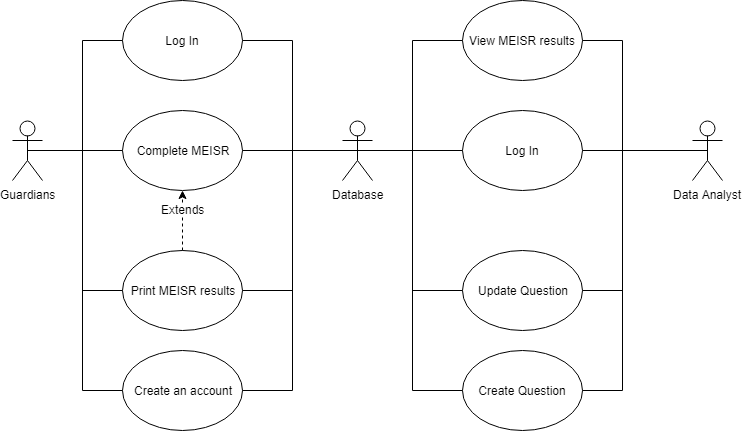
\includegraphics[width=0.7\textwidth]{images/Use_Case_Diagram.png}
  \caption{MEISR Use Case Diagram}
  \label{fig:useCase}
\end{figure}

Figure \ref{fig:useCase} shows three actors who will be interacting with out application. The first and most frequent actor will be the Guardians, or the people who fill out the survey about their children. The Guardian will have the options to Create and Account, Login, Complete MEISR, and Print MEISR Results. The second actor will be the Data Analyst who will query our back-end database to find trends or analyze results. The options available to him will be: Login, View MEISR Results, Update Question, and Create Question.

\section{UML Activity Diagrams}

\subsection{Create Account Activity Diagram}

\begin{figure}[h]
  \centering
  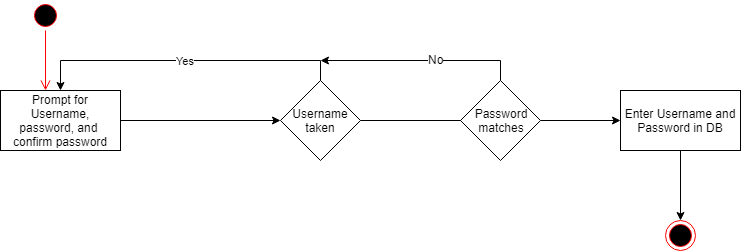
\includegraphics[width=0.7\textwidth]{images/Create_Account_Activity_Diagram.png}
  \caption{Create Account Activity Diagram}
  \label{fig:createAccount}
\end{figure}

Figure \ref{fig:createAccount} shows the process of creating an account. The user is prompted to enter a user name and password then confirm the password. The Database is queried to see if the user name is taken. If user name is free check that the password matches the confirm password. If both conditions are met enter the user name and password combination in the database. Otherwise prompt again.

\subsection{Log In Activity Diagram}

\begin{figure}[h]
  \centering
  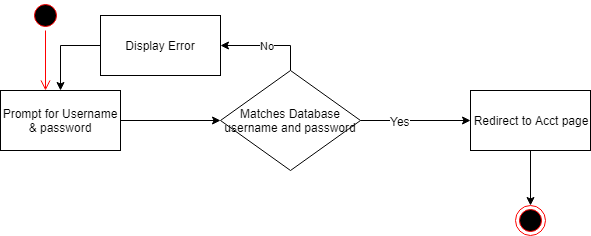
\includegraphics[width=0.7\textwidth]{images/Log_In_Activity_Diagram.png}
  \caption{Log In Activity Diagram}
  \label{fig:logIn}
\end{figure}

Figure \ref{fig:logIn} shows the process of logging in. First, prompt for user name and password. If the user name password combination matches one found in the database redirect to the account page. Otherwise display an error and redirect to the login prompt.

\subsection{Create Question Activity Diagram}

\begin{figure}[h]
  \centering
  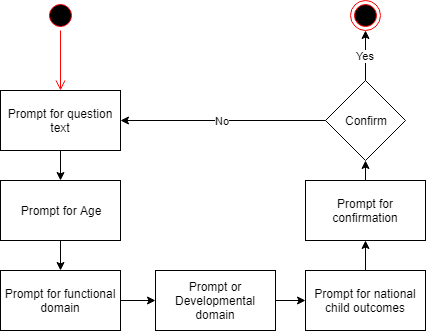
\includegraphics[width=0.7\textwidth]{images/Create_Question_Activity_Diagram.png}
  \caption{Create Question Activity Diagram}
  \label{fig:createQuestion}
\end{figure}

Figure \ref{fig:createQuestion} shows the process of creating a new MEISR question. The process begins by prompting for all necessary question fields (text, age, functional domain, etc.) then ask for confirmation after all information has been entered. If confirmation is given, add to the database. Otherwise redirect to the new question prompts.

\subsection{Update Question Activity Diagram}

\begin{figure}[h]
  \centering
  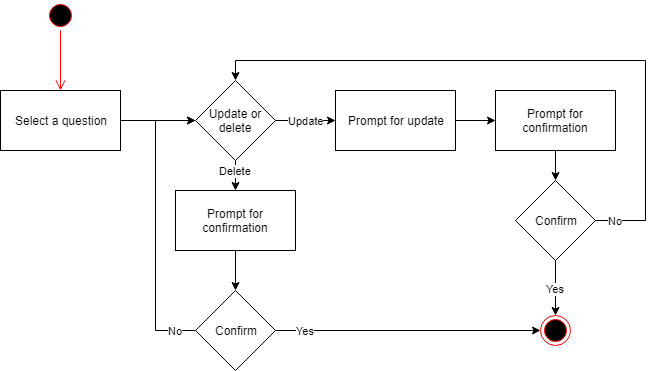
\includegraphics[width=0.7\textwidth]{images/Update_Question_Activity_Diagram.png}
  \caption{Update Question Activity Diagram}
  \label{fig:updateQuestion}
\end{figure}

Figure \ref{fig:updateQuestion} shows the process of updating a question. This process also includes deletion. After selecting a question, choose to update or delete the question. If delete, prompt for confirmation. If update, display all question fields and prompt for update then prompt for confirmation. If confirmed update the database otherwise redirect to update question prompts.

\subsection{Complete MEISR Activity Diagram}

\begin{figure}[h]
  \centering
  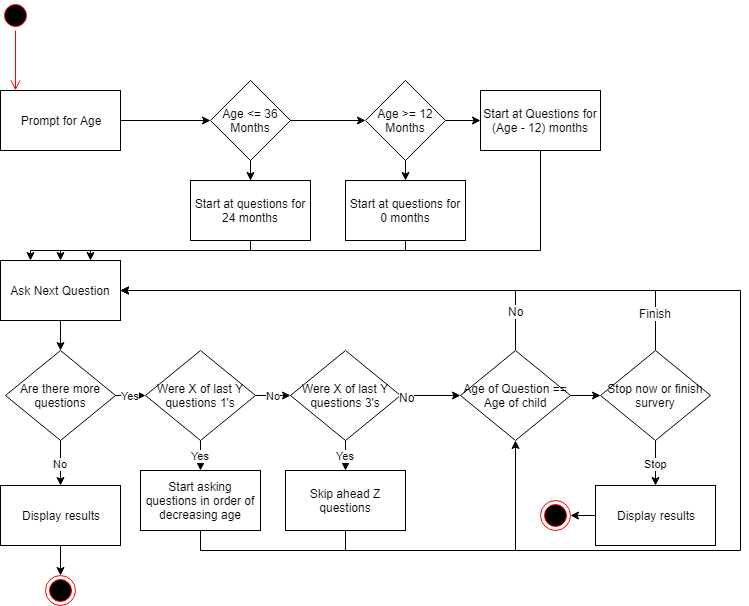
\includegraphics[width=0.7\textwidth]{images/Complete_MEISR_Activity_Diagram.png}
  \caption{Complete MEISR Activity Diagram}
  \label{fig:completeMEISR}
\end{figure}

Figure \ref{fig:completeMEISR} shows the process of completing the MEISR survery. Begin with a prompt for the child's age to determine at what age to start the questions. The questions will skip ahead or move back depending on the answers to previous questions. The questions end when there are no more questions or the parent reaches the child's age and chooses to stop rather than complete the remaining questions.

\subsection{View MEISR Results Activity Diagram}

\begin{figure}[h]
  \centering
  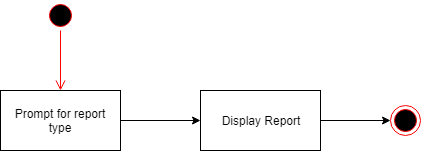
\includegraphics[width=0.7\textwidth]{images/View_MEISR_Results_Activity_Diagram.png}
  \caption{View MEISR Results Activity Diagram}
  \label{fig:viewMEISRResults}
\end{figure}
  
  Figure \ref{fig:viewMEISRResults} shows the process of displaying results for a completed MEISR survey. The user will select a report type from a selection of pre\-generated reports, and the report will display.
  
\section{UML High Level Class Diagram}

\begin{figure}[h]
  \centering
  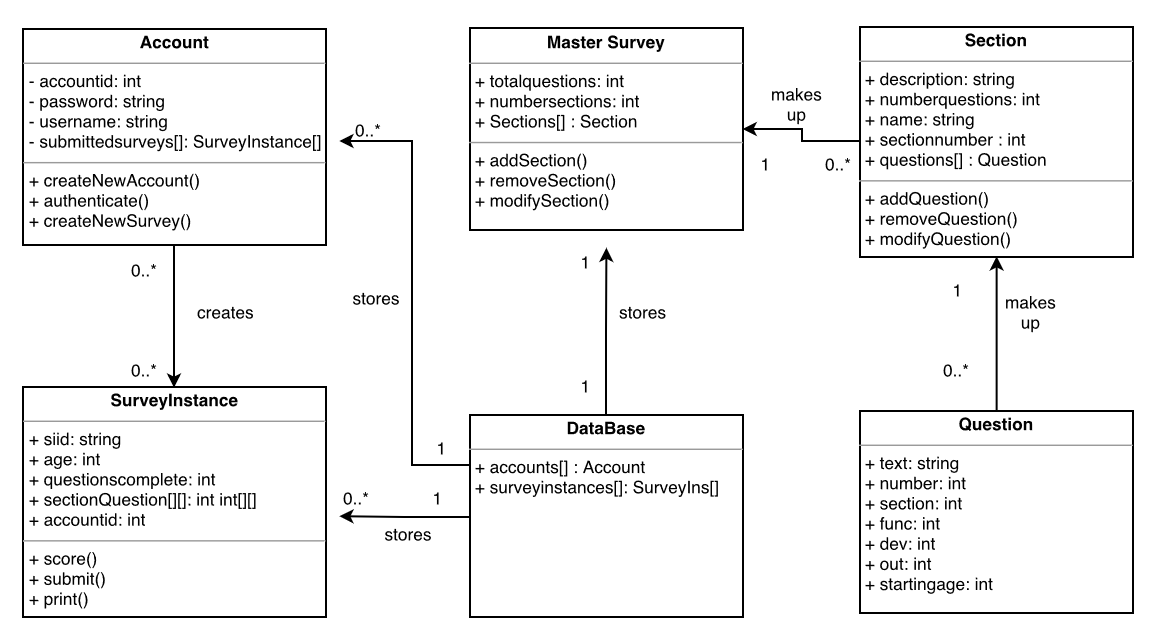
\includegraphics[width=0.7\textwidth]{images/HighLevelClassDiagramCS495.png}
  \caption{UML High Level Class Diagram}
  \label{fig:classDiagram}
\end{figure}

The classes we have proposed revolved around 3 main areas shown in figure \ref{fig:classDiagram}. First there is the Master Survey Class that contains the information about the current MEISR survey. If the current MEISR needs to be updated then the Master Survey Class is responsible for containing/changing that information. Second is the Account and Survey Instance class. This are both objects which will be created and stored in the database by users. This data can then be accessed later by researchers and clients. Lastly, the third area is the database itself, which needs to store accounts, surveys, and the master list.


Account Class
	The account class is created by a user when he first starts the app. It contains basic information such as username and password. It also contains a unique identification number, and all SurveyInstance objects created by this particular user in an Array.

SurveyInstance:
	An object of this class is created when the user starts a new MEISR survey. This class contains information such as the age of the child, how many questions have been completed, and it keeps track of the answers to that particular survey.

Question Class:
	This class contains the information needed to make a question such as text, number, description, ect. A question object is created and then added to an array of question objects in the section class.

Section Class:
	This class contains the information needed to make a section such as, section title, description, number, and all the questions contained in that section.

Master Survey:
	This class contains the information about the most up to date version of the MEISR, such as number of questions, number of sections, and an array of section objects, which contain the questions.

DataBase Class:
	This is not necessarily a class we will code, but it represents the entity of the database and how it interacts with our proposed system. We think we implement an SQL database as the information we need to store is mostly uniform. We also think that the SQL database will scale better with large tables versus querying large numbers of documents in a noSQL database.



\begin{appendices}
%%%%%%%% GLOSSARY %%%%%%%%%
\chapter{Glossary}
\textbf{MEISR}: An acronym for “Measure of Engagement, Independence, and Social Relationships”, a survey created by Dr. McWilliam of EIEIO for the purpose of evaluating child development in the categories named as they grow.\\
\textbf{MEISR App}: The translation of the MEISR to an Android application with the purpose of providing a more powerful experience to users.\\
\textbf{Guardian}: A parent or primary caretaker of a child with a disability who is expected to be the primary operator of the app.\\
\textbf{Disability}: A documented case of some mental disability diagnosed by a psychological professional.\\
\textbf{Analyst}: A professional given access to the raw data collected by the MEISR app for the purpose of statistical analysis.\\
\textbf{Android}: A mobile operating system developed by Google based on the Linux operating system and other open source softwares.\\
\textbf{Android SDK}: a software development tool that provides APIs for creating Android apps using the Java programming language.\\
\textbf{API}: An acronym for “application programming interface”, a set of subroutines, protocols, and tools for building a software application.\\
%%%%%%%%%%%%%%%%%%%%%%
\end{appendices}


